      \begin{figure*}
        \centering
        \begin{subfigure}[b]{0.35\textwidth}
            \centering
            \caption[]%
            {{Netpipe:64 KB Message}}  
            \vspace*{-0.25cm}  
            \label{fig:joule_netpipe64}
            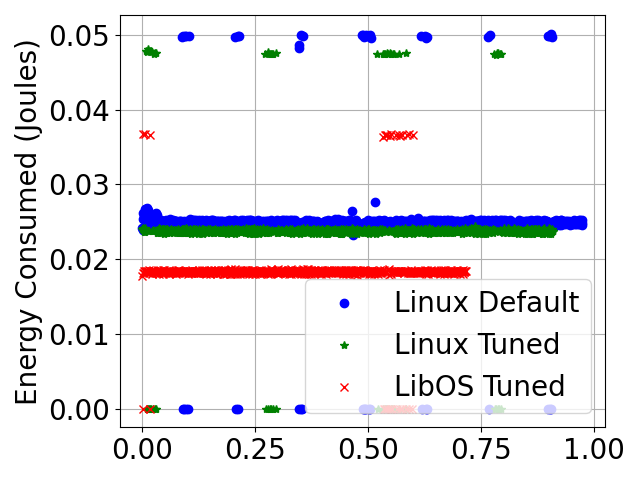
\includegraphics[width=\textwidth]{osdi_figures/netpipe_65536_joule_timeline.png}
        \end{subfigure}
     %   \hfill
        \begin{subfigure}[b]{0.35\textwidth}  
            \centering 
            \caption[]%
            {{Memcached:600K QPS}} 
            \vspace*{-0.25cm}    
            \label{fig:joule_mcd600}
            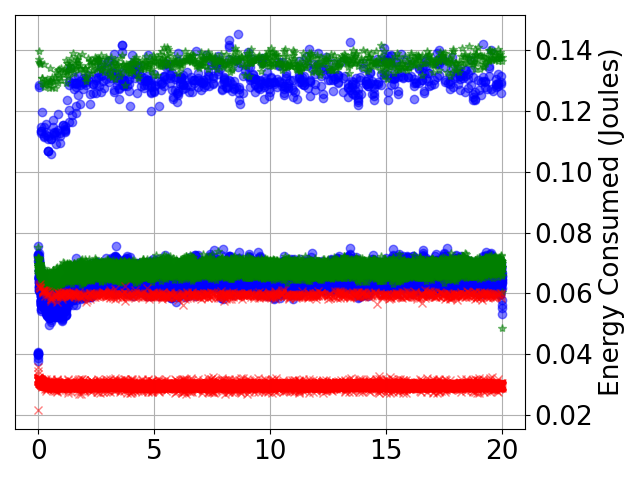
\includegraphics[width=\textwidth]{osdi_figures/mcd_600000_joules_timeline.png}
        \end{subfigure}
        \vskip\baselineskip
        \vspace*{-0.62cm} 
        \begin{subfigure}[b]{0.35\textwidth}   
            \centering 
            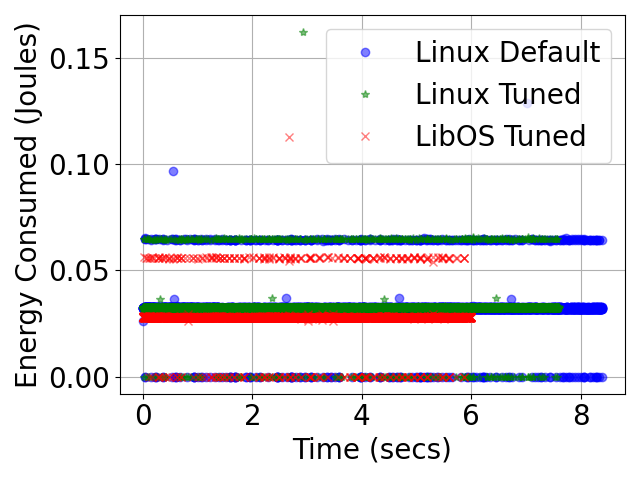
\includegraphics[width=\textwidth]{osdi_figures/nodejs_joule_timeline.png}
            \caption[]%
            {{NodeJS}}    
            \label{fig:joule_nodejs}
        \end{subfigure}
       % \hfill
        \begin{subfigure}[b]{0.35\textwidth}   
            \centering 
            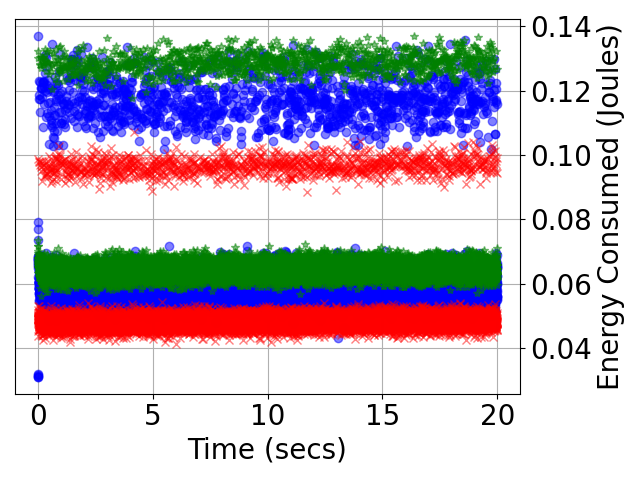
\includegraphics[width=\textwidth]{osdi_figures/mcdsilo_200000_joules_timeline.png}
            \caption[]%
            {{Memcached-silo:200K QPS}}    
            \label{fig:joule_mcdsilo200}
        \end{subfigure}
        \caption[]
        {Energy timelines from selected runs:  Joule difference between every 1 ms reading of joule register plotted against time of entire experimental run.} 
        \label{fig:joule}
    \end{figure*}%  
